\documentclass[10pt,a4paper]{article}
\usepackage[utf8]{inputenc}
\usepackage[english]{babel}
\usepackage{amsmath}
\usepackage{amsfonts}
\usepackage{amssymb}
\usepackage{graphicx}
\usepackage{subfigure}
\usepackage[left=2cm,right=2cm,top=2cm,bottom=2cm]{geometry}
%===============CODE LISTING=======================
\usepackage{listings}
\usepackage{xcolor} % for setting colors

%Define custom colors
\definecolor{dkgreen}{rgb}{0,0.6,0}
\definecolor{gray}{rgb}{0.5,0.5,0.5}
\definecolor{mauve}{rgb}{0.58,0,0.82}
\definecolor{backcolour}{rgb}{0.95,0.95,0.92}

%Define style and language
\lstset{ 
  language=SQL,            % the language of the code (TeX) and its dialect (LaTeX). If dialect is not specified, the package chooses the default dialect
  basicstyle=\footnotesize,       % the size of the fonts that are used for the code
  numbers=left,                   % where to put the line-numbers
  numberstyle=\tiny\color{gray},  % the style that is used for the line-numbers
  stepnumber=1,                   % the step between two line-numbers. If it's 1, each line will be numbered
  numbersep=5pt,                  % how far the line-numbers are from the code
  backgroundcolor=\color{backcolour},  % choose the background color. You must add \usepackage{color}
  showspaces=false,               % show spaces adding particular underscores
  showstringspaces=false,         % underline spaces within strings
  showtabs=false,                 % show tabs within strings adding particular underscores
  %frame=single,                   % adds a frame around the code
  rulecolor=\color{black},        % if not set, the frame-color may be changed on line-breaks within not-black text (e.g. commens (green here))
  tabsize=4,                      % sets default tabsize to 2 spaces
  captionpos=b,                   % sets the caption-position to bottom
  breaklines=true,                % sets automatic line breaking
  breakatwhitespace=false,        % sets if automatic breaks should only happen at whitespace
  %title=\lstname,                 % show the filename of files included with \lstinputlisting;
  keywordstyle=\color{blue}\scshape,          % keyword style
  commentstyle=\color{dkgreen},       % comment style
  stringstyle=\color{orange},         % string literal style
  %escapeinside={\%*}{*)},            % if you want to add a comment within your code
  morekeywords={format}               % if you want to add more keywords to the set
}
%=================================
\author{Huy Bui}
\begin{document}
\begin{tabular}{p{8cm}l}
	\textbf{Huy Bui}		&	\textsc{DATABASE}			\\
	Information Technology	&	\textbf{Simple queries}	\\
	T5616SN					&	\today				\\
\end{tabular}
\section{Query in SQL}
The purpose of this article is to lay out the basic structure and use of SQL SELECT queries and statements. These statements are part of Transact-SQL (T-SQL) language specification and are central to the use of Microsoft SQL Server.\par 
Once we have data in the database, we want to look at the data and analyze it in an endless number of different ways, constantly varying the filtering, sorting, and calculations that we apply to the raw data. The SQL SELECT statement is what we use to choose, or select, the data that we want returned from the database to our application.
\subsection{The SELECT ... FROM clause}
The most basic SELECT statement has only 2 parts: (1) what columns you want to return and (2) what table(s) those columns come from. If we want to retrieve all of the information about all of the customers in the Employees table, we could use the asterisk (*) as a shortcut for all of the columns, and our query looks like
\begin{lstlisting}
	SELECT * FROM Employees
\end{lstlisting}
If we want only specific columns (as is usually the case), we can/should explicitly specify them in a comma-separated list, as in
\begin{lstlisting}
	SELECT EmployeeID, FirstName, LastName, HireDate, City FROM Employees
\end{lstlisting}
which results in the specified fields of data for all of the rows in the table:
\begin{figure}[hbtp]
	\centering
	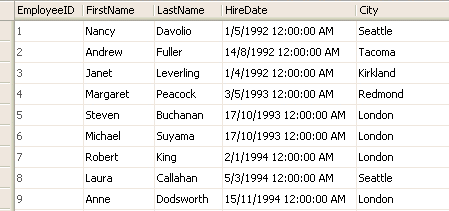
\includegraphics[scale=1]{example.png}
	\caption{Select multiple columns}
	\end{figure}
 
\subsection{The WHERE clause}
The next thing we want to do is to start limiting, or filtering, the data we fetch from the database. By adding a WHERE clause to the SELECT statement, we add one (or more) conditions that must be met by the selected data. This will limit the number of rows that answer the query and are fetched. In many cases, this is where most of the "action" of a query takes place. We can continue with our previous query, and limit it to only those employees living in London:
\begin{lstlisting}
	SELECT EmployeeID, FirstName, LastName, HireDate, City FROM Employees
	WHERE City = 'London'
	\end{lstlisting}
\begin{figure}[hbtp]
	\centering
	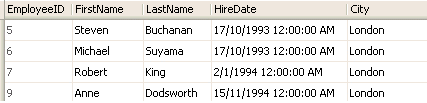
\includegraphics[scale=1]{WhereClause.png}
	\caption{List all employees living in London using WHERE clause}
	\end{figure}

\subsection{The ORDER BY clause}
Until now, we have been discussing filtering the data: that is, defining the conditions that determine which rows will be included in the final set of rows to be fetched and returned from the database. Once we have determined which columns and rows will be included in the results of our SELECT query, we may want to control the order in which the rows appear—sorting the data. To sort the data rows, we include the ORDER BY clause. The ORDER BY clause includes one or more column names that specify the sort order. If we return to one of our first SELECT statements, we can sort its results by City with the following statement:
\begin{lstlisting}
	SELECT EmployeeID, FirstName, LastName, HireDate, City FROM Employees
	ORDER BY City
	\end{lstlisting}
\begin{figure}[hbtp]
	\centering
	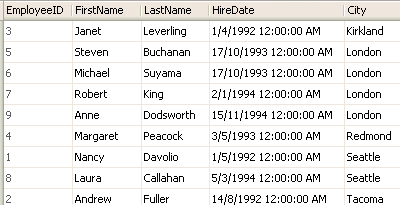
\includegraphics[scale=1]{Order.png}
	\caption{Sort results by City}
	\end{figure}

\subsection{The GROUP BY clause}
The GROUP BY clause groups the SELECT statement results according to the values in a list of one or more column expressions. For example, consider the Sales table ().\\
\begin{tabular}{|l|l|l|}
	\hline 
	\textbf{Country} & \textbf{Region} & \textbf{Sales} \\ 
	\hline 
	Canada & Alberta & 100 \\ 
	\hline 
	Canada & British Columbia & 200 \\ 
	\hline 
	Canada & British Columbia & 300 \\ 
	\hline 
	United States & Montana & 100 \\ 
	\hline 
	\end{tabular} \\
This next query groups Country and Region and returns the aggregate sum for each combination of values. 
\begin{lstlisting}
	SELECT Country, Region, SUM(sales) AS TotalSales
	FROM Sales
	GROUP BY Country, Region;
	\end{lstlisting}
The GROUP BY clause also interacts with other statements, such as COUNT, AVG, HAVING. As for HAVING clause, it searchs condition for a group or an aggregate. COUNT returns the number of items in a group. And AVG returns the average of the values in a group. 

\section{Practical part}
The following query lists all staff with age greater than 50 years including at columns FirstName, FamilyName, and DateOfBirth from Staff table (Figure \ref{1-50years}).
\lstinputlisting{1-50years.sql}
\begin{figure}[hbtp] 
	\centering
	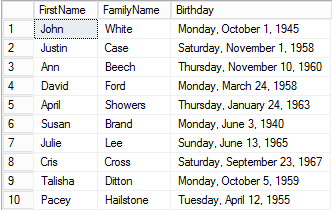
\includegraphics[scale=1]{1-50years.PNG}
	\caption{Older-than-50 staffs and their birthday}
	\label{1-50years}
	\end{figure}
The following query produces a list of monthly salary for all staff, showing first and last names, and salary details, and annual salary information in table Staff (Figure \ref{2-Salary}).
\lstinputlisting{2-Salary.sql}
\begin{figure}[hbtp]
	\centering
	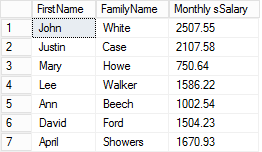
\includegraphics[scale=1]{2-Salary.PNG}
	\caption{Show monthly salary for all staff}
	\label{2-Salary}
	\end{figure}
The following query find all owners who live in Glasgow. Include at least FirstName, FamilyName, and City from PrivateOwner table in your result table (Figure \ref{3-Glasgow}).
\lstinputlisting{3-Glasgow.sql}
\begin{figure}[hbtp]
	\centering
	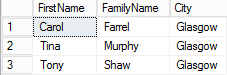
\includegraphics[scale=1]{3-Glasgow.PNG}
	\caption{Show all staffs who live in Glasgow}
	\label{3-Glasgow}
	\end{figure}
The following query produces a list of all staff, arranged in alphabetical order of first name (Figure \ref{4-OrderFirstName}).
\lstinputlisting{4-OrderFirstName.sql}
\begin{figure}[hbtp]
	\centering
	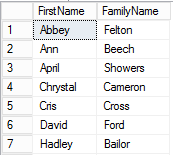
\includegraphics[scale=1]{4-OrderFirstName.PNG}
	\caption{Show staffs' names in alphabetical order}
	\label{4-OrderFirstName}
	\end{figure}
The following query produces a list of all staff, arranged in order of age (Figure \ref{4-OrderAge}).
\lstinputlisting{4-OrderAge.sql}
\begin{figure}[hbtp]
	\centering
	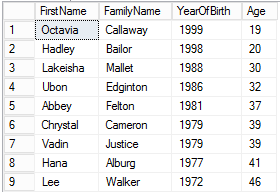
\includegraphics[scale=1]{4-OrderAge.PNG}
	\caption{Show staffs' ages in ascending order}
	\label{4-OrderAge}
	\end{figure}
The following query produces a list of properties for rent in order of property type (major sort
key) in ascending alphabetic order, and within property type, in descending order of rent (minor sort key) (Figure \ref{5-OrderProperty}).
\lstinputlisting{5-OrderProperty.sql}
\begin{figure}[hbtp]
	\centering
	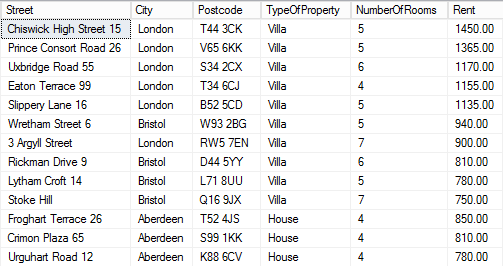
\includegraphics[scale=1]{5-OrderProperty.PNG}
	\caption{Sort list in order of property type and rent}
	\label{5-OrderProperty}
	\end{figure}
The following query lists the number of properties in each property type (Figure \ref{6-Number-properties}).
\lstinputlisting{6-Number-properties.sql}
\begin{figure}[hbtp]
	\centering
	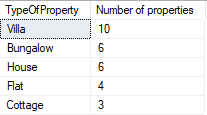
\includegraphics[scale=1]{6-Number-properties.PNG}
	\caption{Sort list in order of property type and rent}
	\label{6-Number-properties}
	\end{figure}
The following query lists the number of properties managed by each staff member (Figure \ref{7-properties-staff}).
\lstinputlisting{7-properties-staff.sql}
\begin{figure}[hbtp]
	\centering
	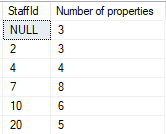
\includegraphics[scale=1]{7-properties-staff.PNG}
	\caption{Sort list in order of property type and rent}
	\label{7-properties-staff}
	\end{figure}
The following query lists the number of properties viewed more than once as well as the number of viewing (Figure \ref{8-Number-viewings}).
\lstinputlisting{8-Number-viewings.sql}
\begin{figure}[hbtp]
	\centering
	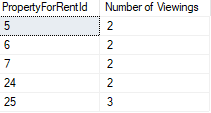
\includegraphics[scale=1]{8-Number-viewings.PNG}
	\caption{Sort list in order of property type and rent}
	\label{8-Number-viewings}
	\end{figure}
The following query shows average rent for each property type (Figure \ref{9-Average-rent}).
\lstinputlisting{9-Average-rent.sql}
\begin{figure}[hbtp]
	\centering
	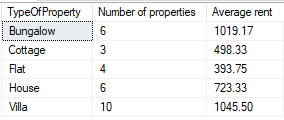
\includegraphics[scale=1]{9-Average-rent.PNG}
	\caption{Sort list in order of property type and rent}
	\label{9-Average-rent}
	\end{figure}
\end{document}